\chapter{Data Exploration}


In the following, we explore some elementary properties of the $225134$ documents in our dataset. The linguistic properties are made on the full-length documents ($3200$ characters).

\subsubsection{Genre Distribution}

\begin{figure}[h]
	\centering
	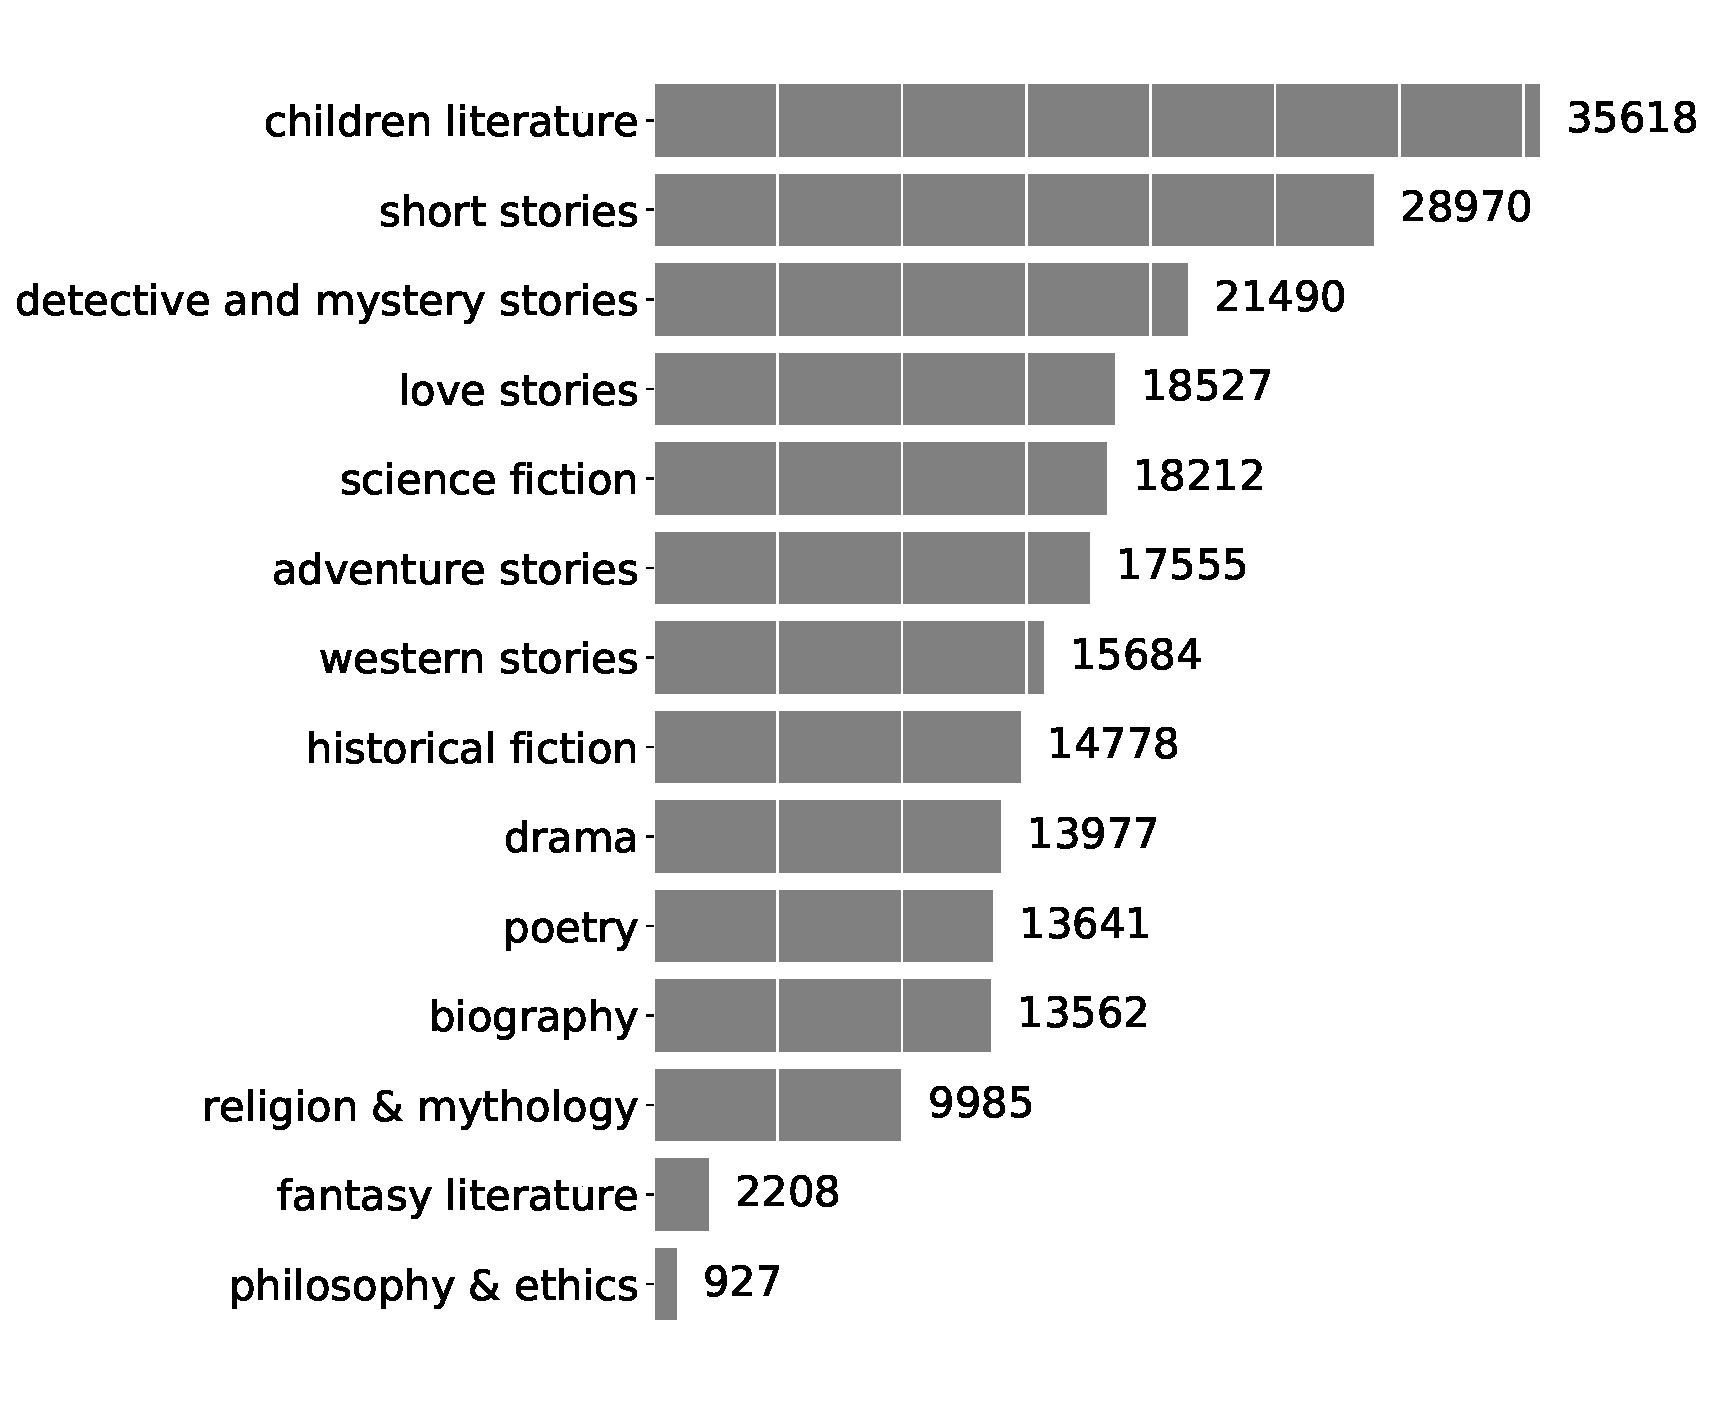
\includegraphics[height=0.4\textheight]{img/03_01_genre_distribution}
	\caption{Genre distribution among documents.}
	\label{fig:genre_distribution}
\end{figure}




\begin{comment}

\subsubsection{Average Word Length}
\begin{itemize}
    \item How do we define word
    \item Distribution per genre
\end{itemize}
\begin{figure}[h]
	\centering
	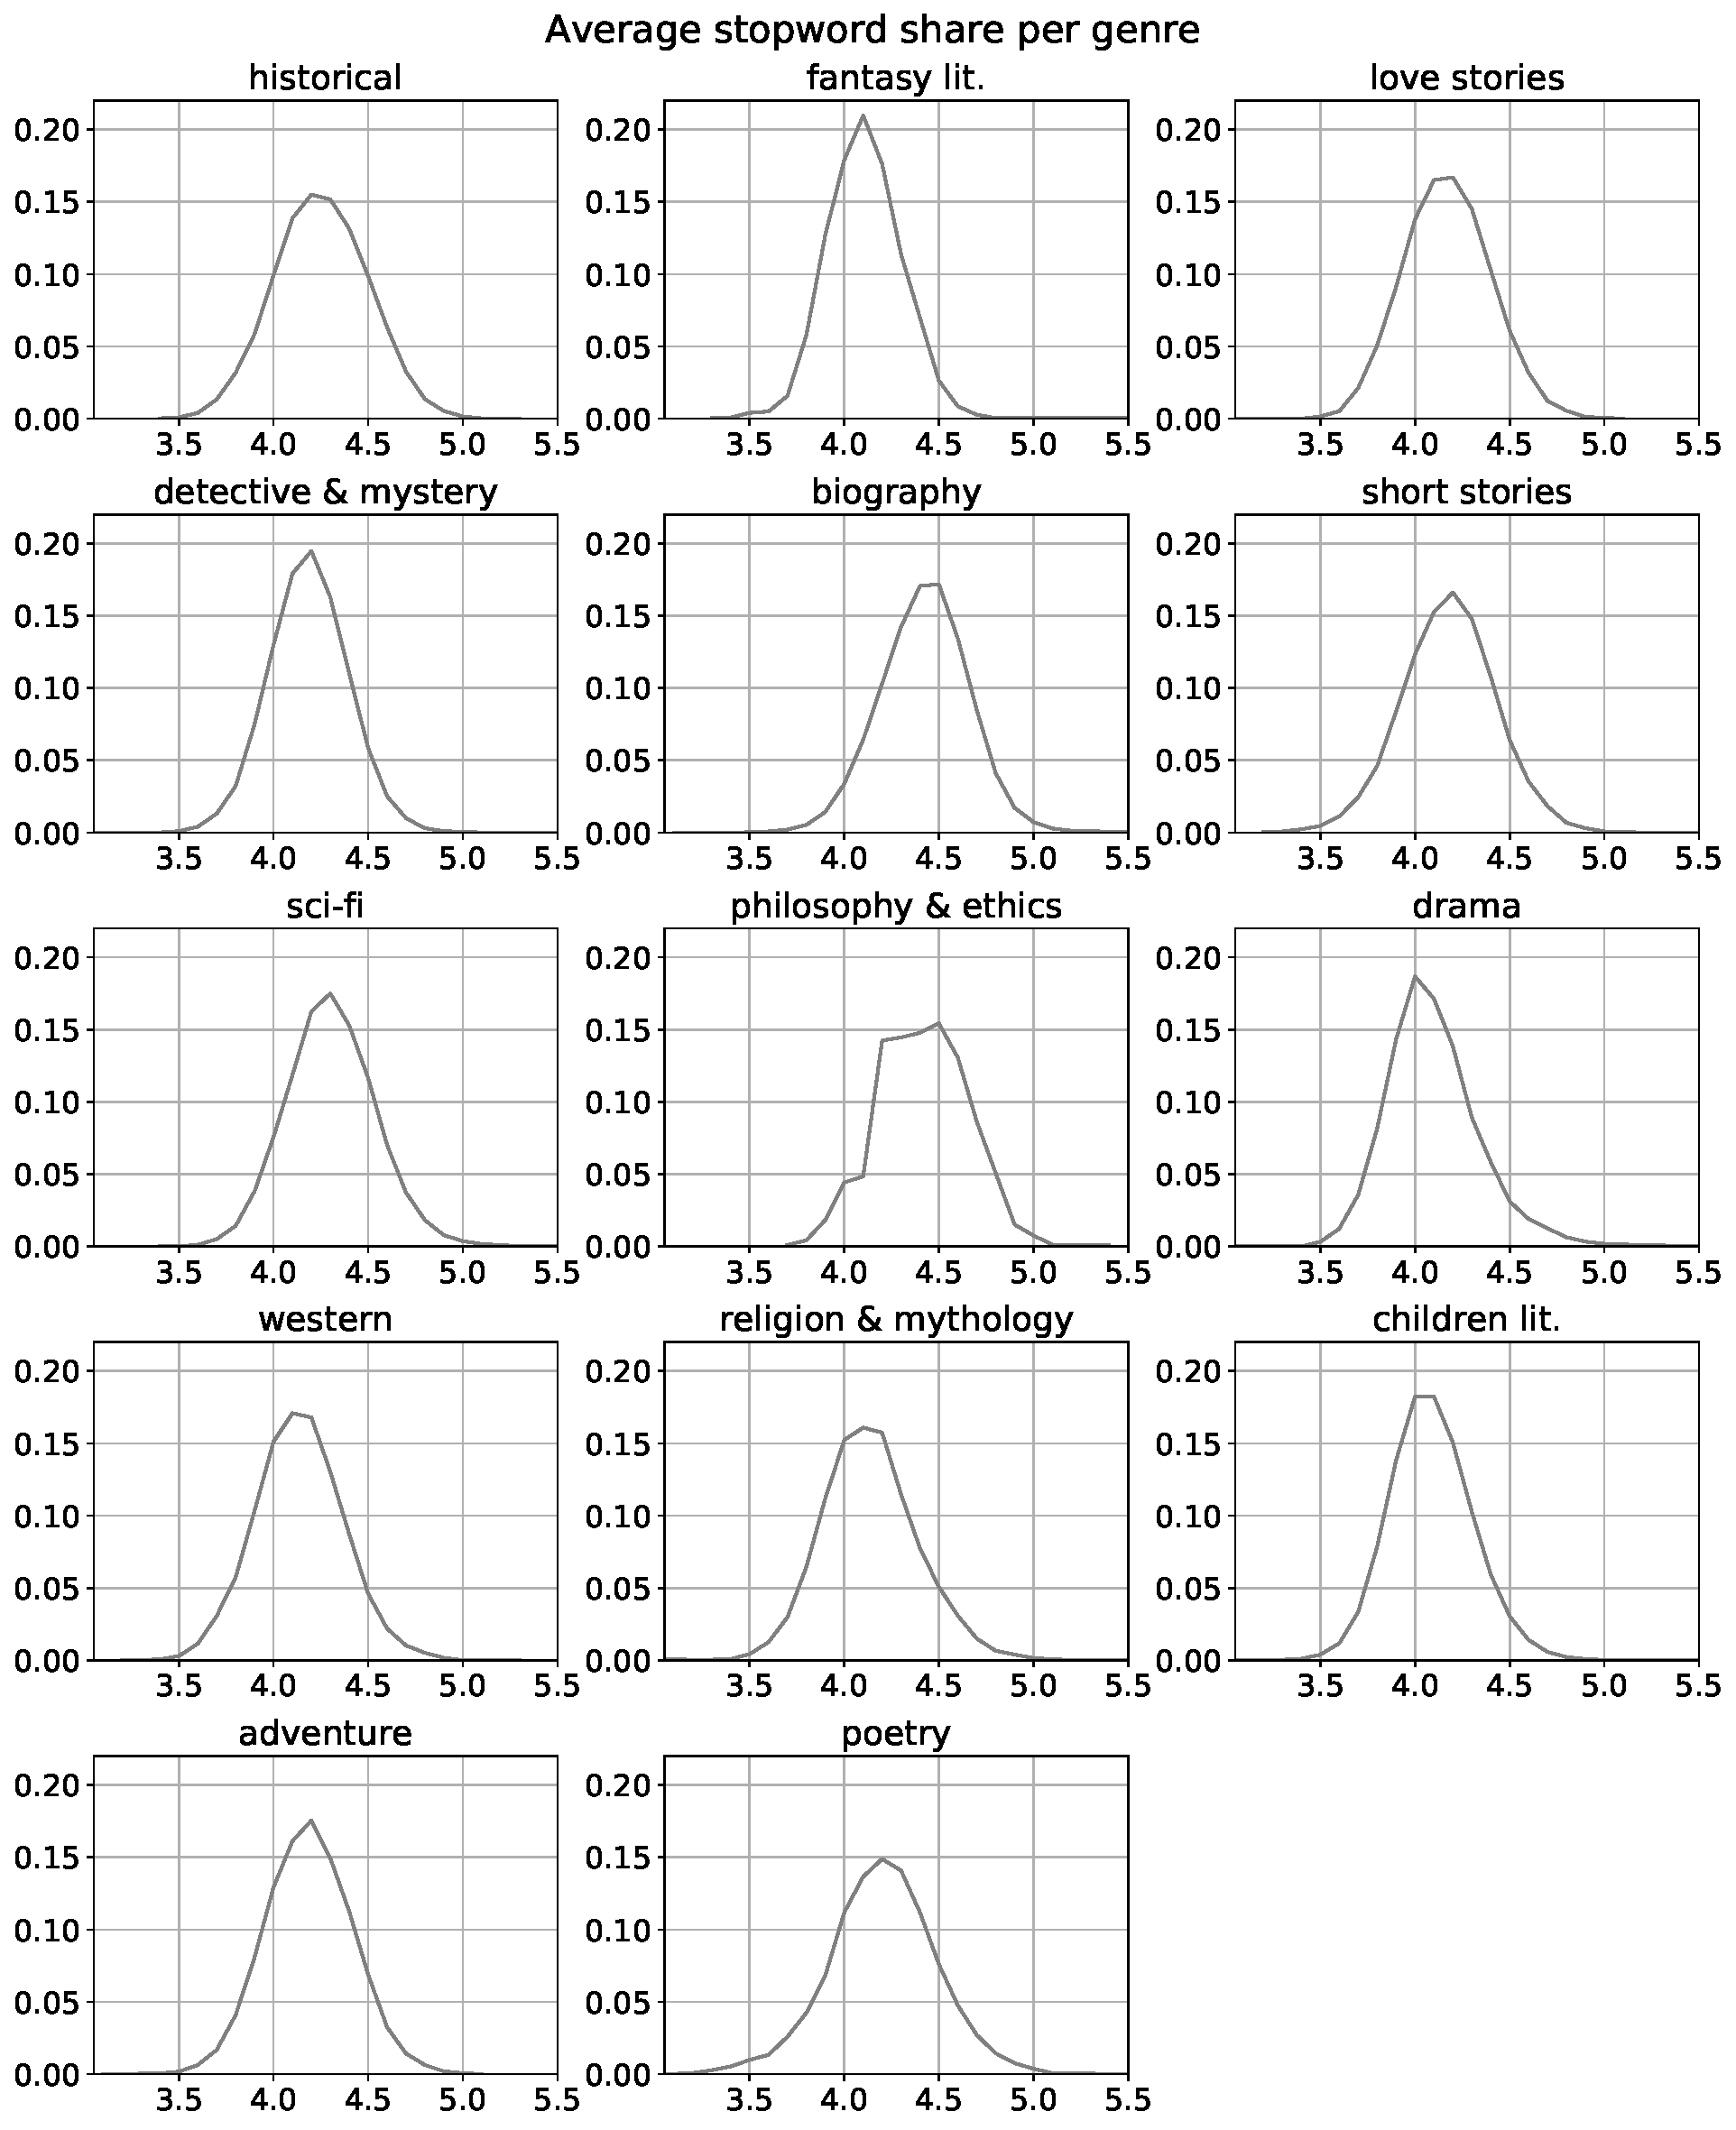
\includegraphics[height=0.4\textheight]{img/03_avg_word_length}
	\caption{Average word length per genre.}
	\label{fig:avg_word_length}
\end{figure}

%%%%%%%%%%%%%%%%%%
%%% SUBFIGURES %%%
%%%%%%%%%%%%%%%%%%

\begin{figure}
\centering

\begin{subfigure}[t]{.5\textwidth}
	\centering
	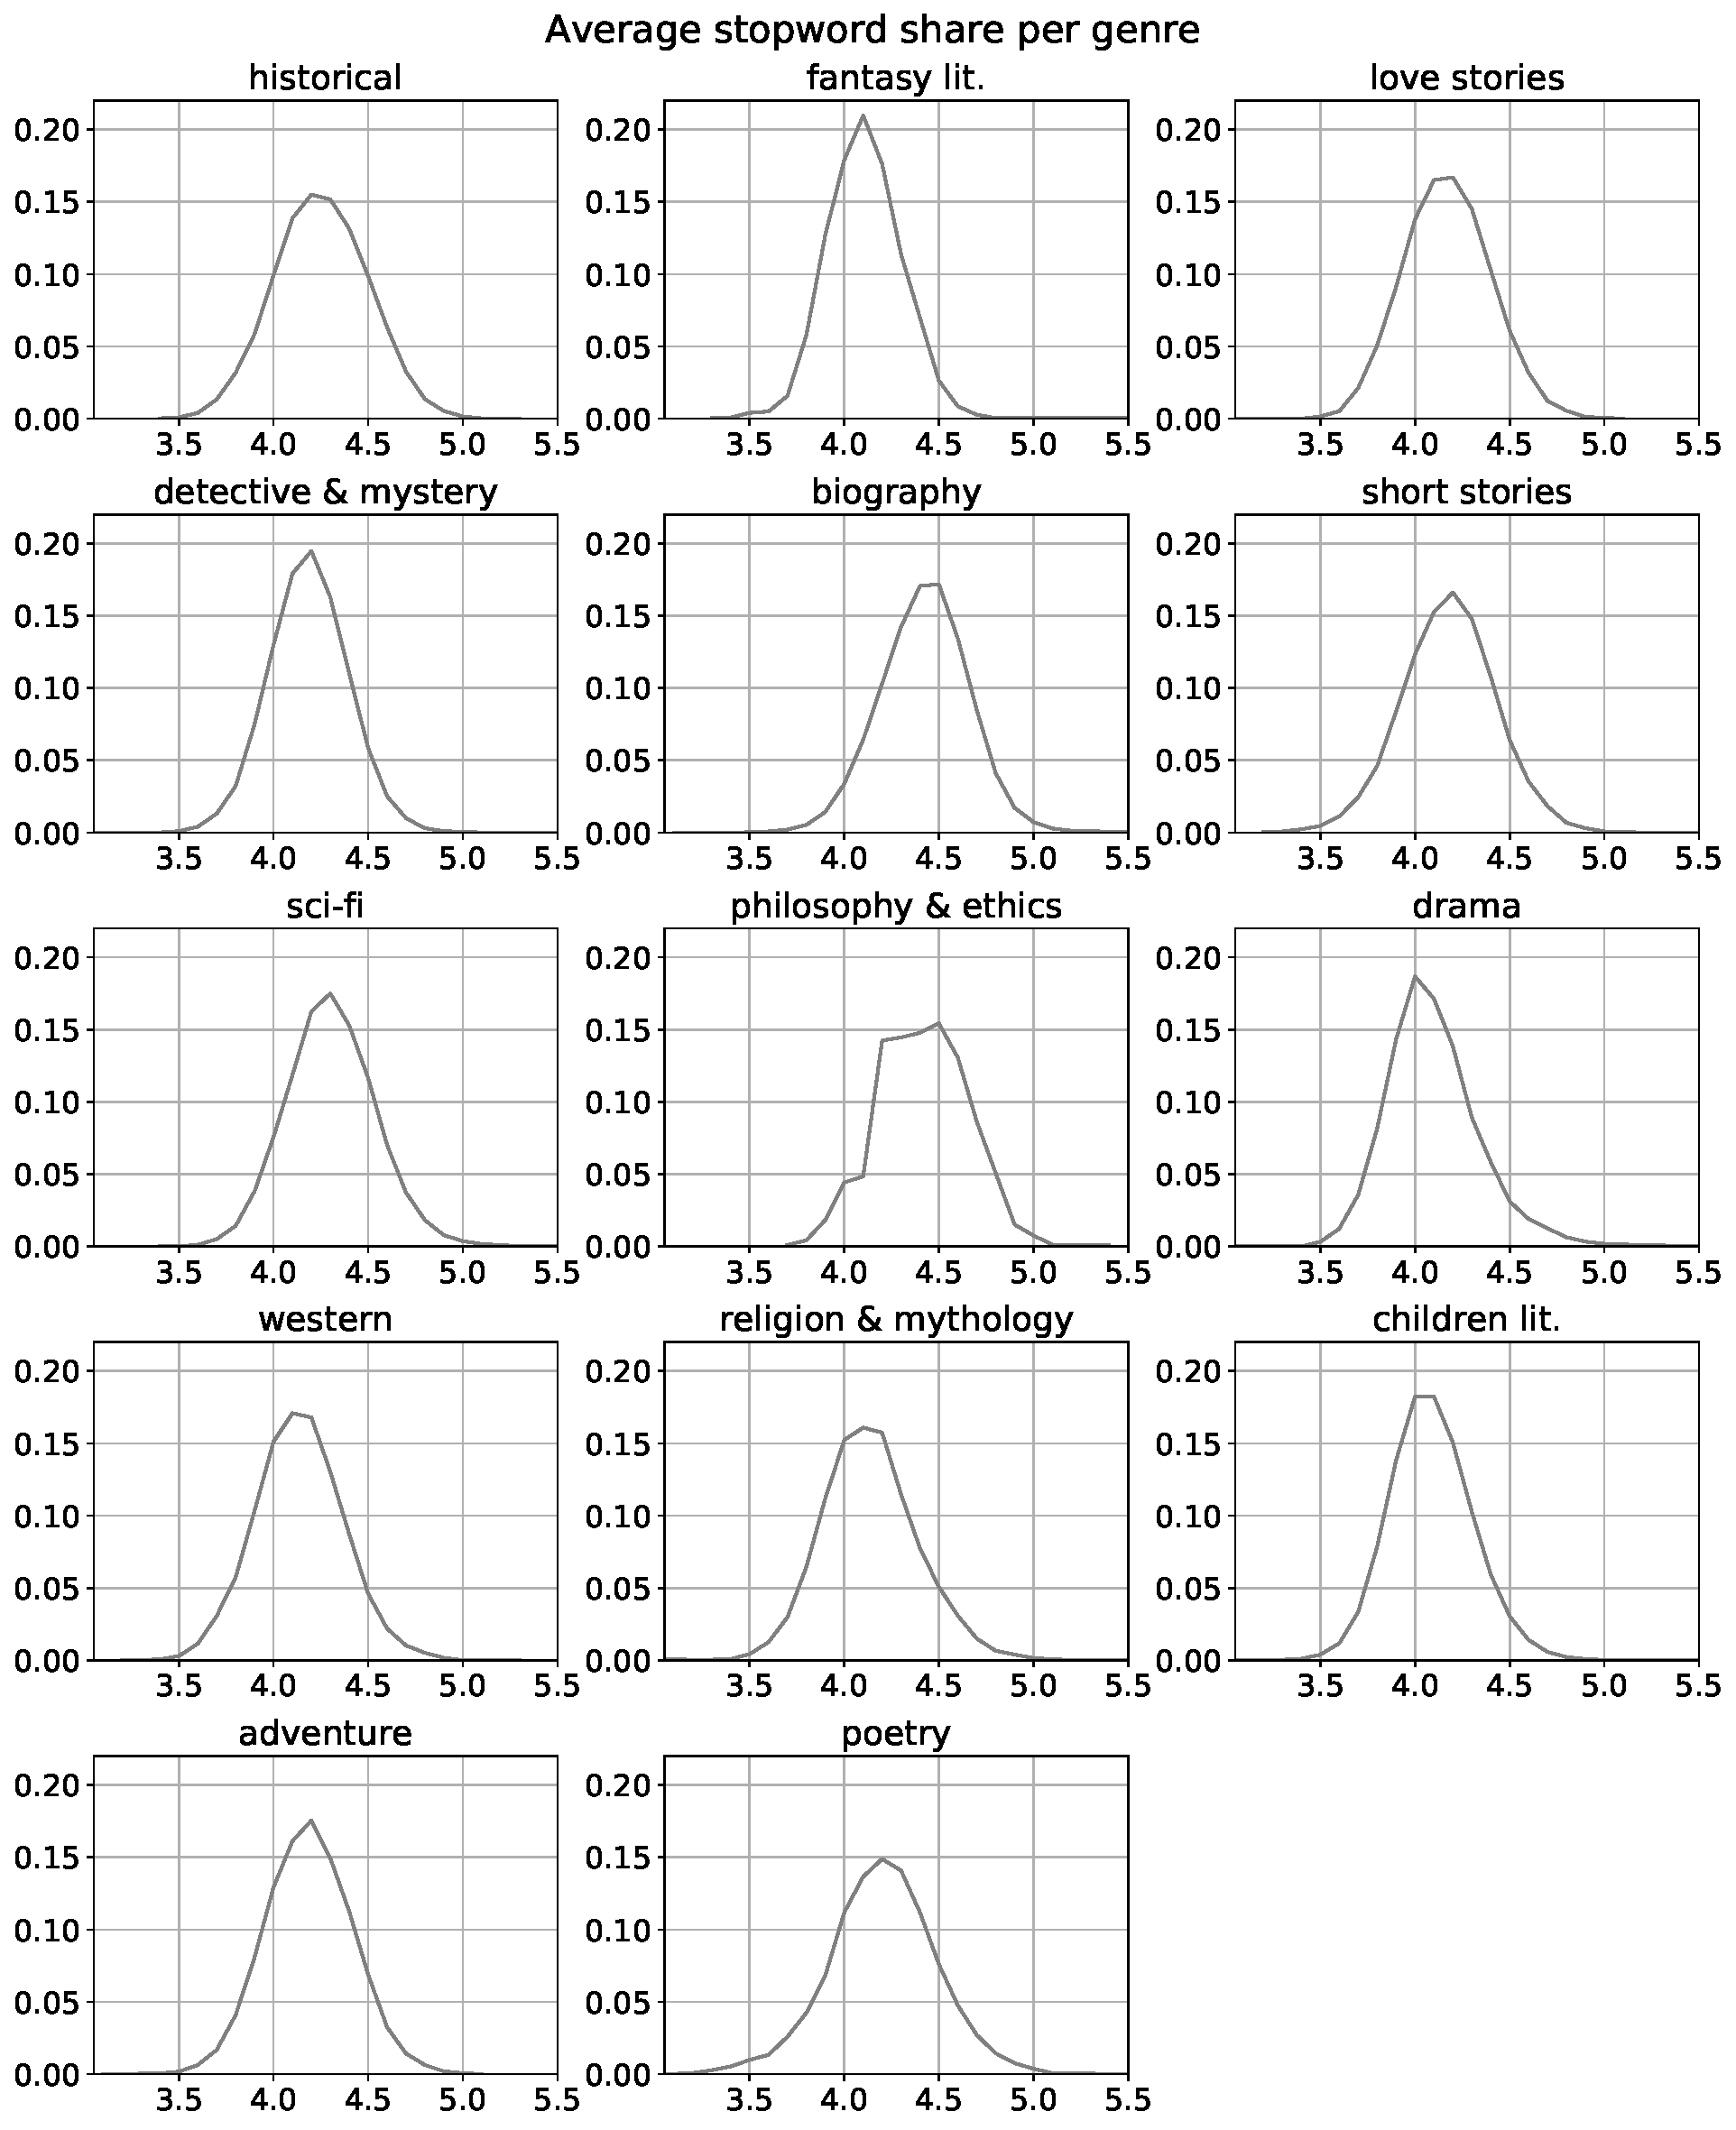
\includegraphics[width=.95\linewidth]{img/03_avg_word_length}
	\caption{Average word length per genre.}
	\label{fig:avg_word_length}
\end{subfigure}%
\begin{subfigure}[t]{.5\textwidth}
	\centering
	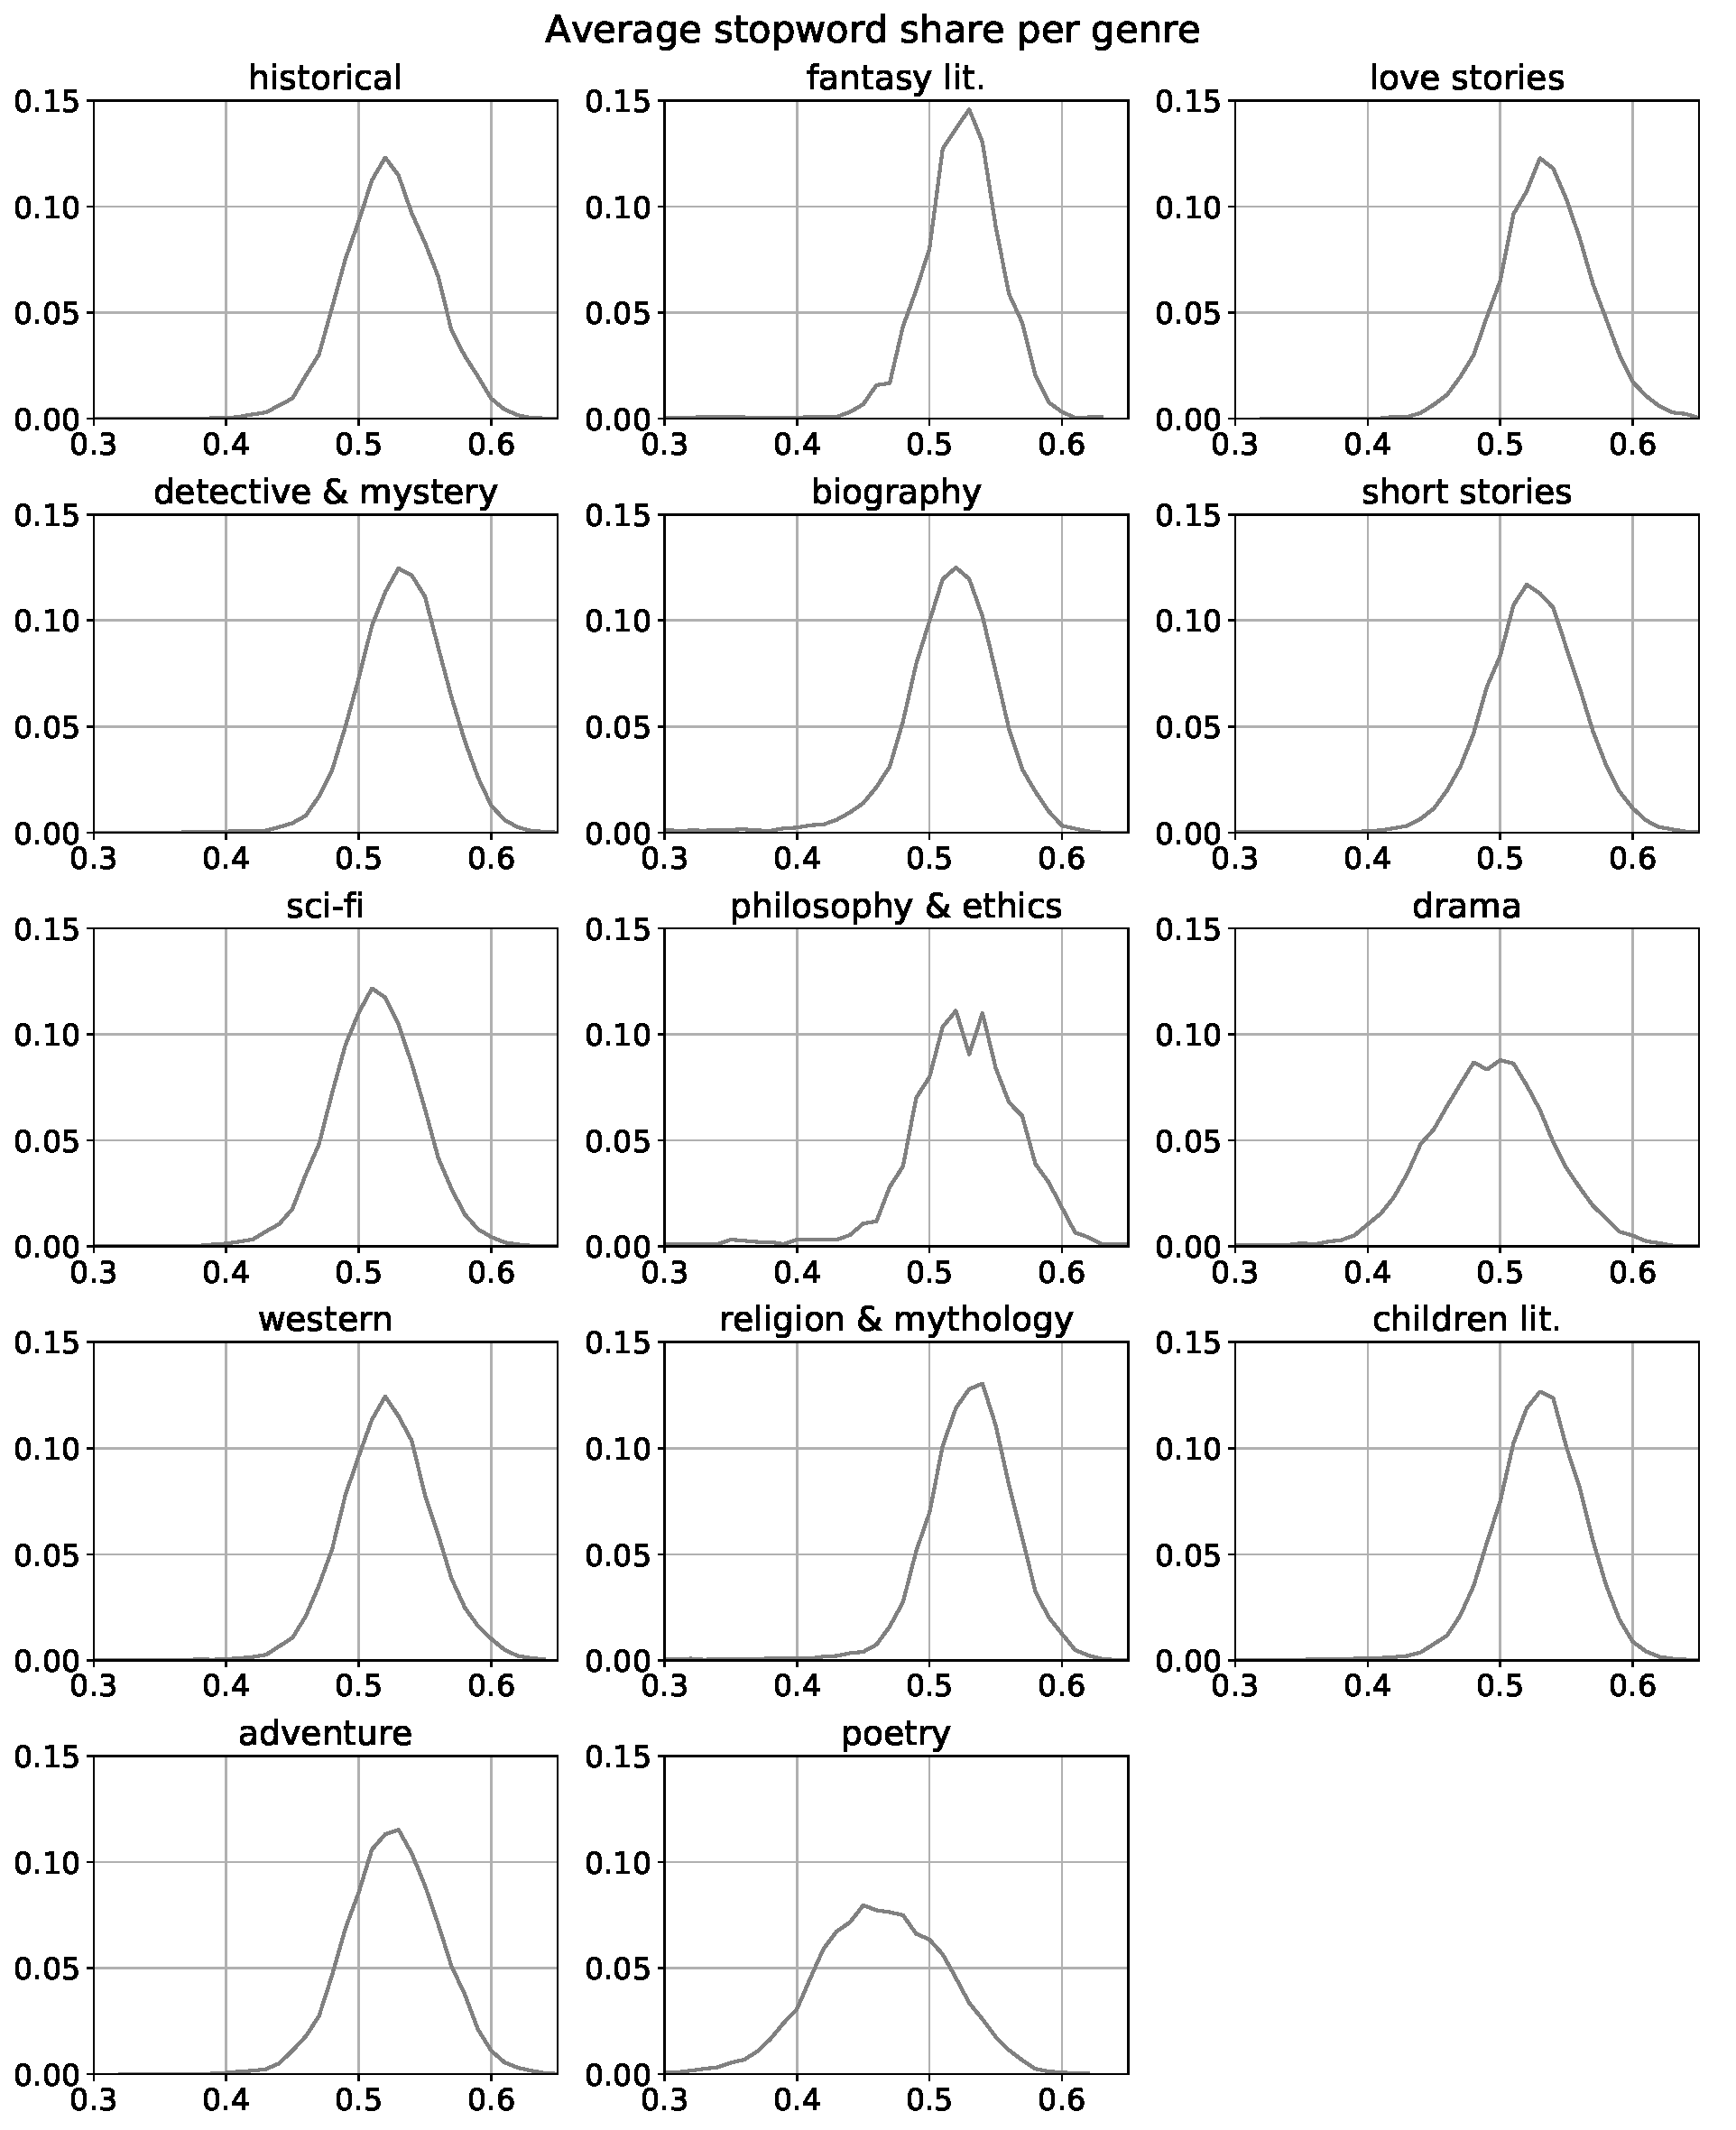
\includegraphics[width=.95\linewidth]{img/03_stopwords}
	\caption{Average stopwords share per genre.}
	\label{fig:stopwords}
\end{subfigure}
\caption{X}
\end{figure}


\end{comment}




\begin{comment}
\begin{tabular}{cc}
  Table head & Table head\\
  Some values & Some values\\
  Some values & Some values\\
  Some values & Some values\\
  Some values & Some values\\
\end{tabular}
\end{comment}

\begin{comment}
\subsubsection{Author Distribution}
\begin{itemize}
    \item How many authors
    \item Snippets per author distribution
    \item Main authors
\end{itemize}

\subsubsection{Average Sentence Length}
\begin{itemize}
    \item How do we define sentence
    \item Distribution per genre
\end{itemize}
\end{comment}
% Readability measures - https://pypi.org/project/ReadabilityCalculator





\begin{comment}


\subsubsection{Stop Words Proportion}
Stop words definition as in \texttt{nltk.corpus.stopwords}. Examples of what stopwords are in.
\begin{figure}[h]
	\centering
	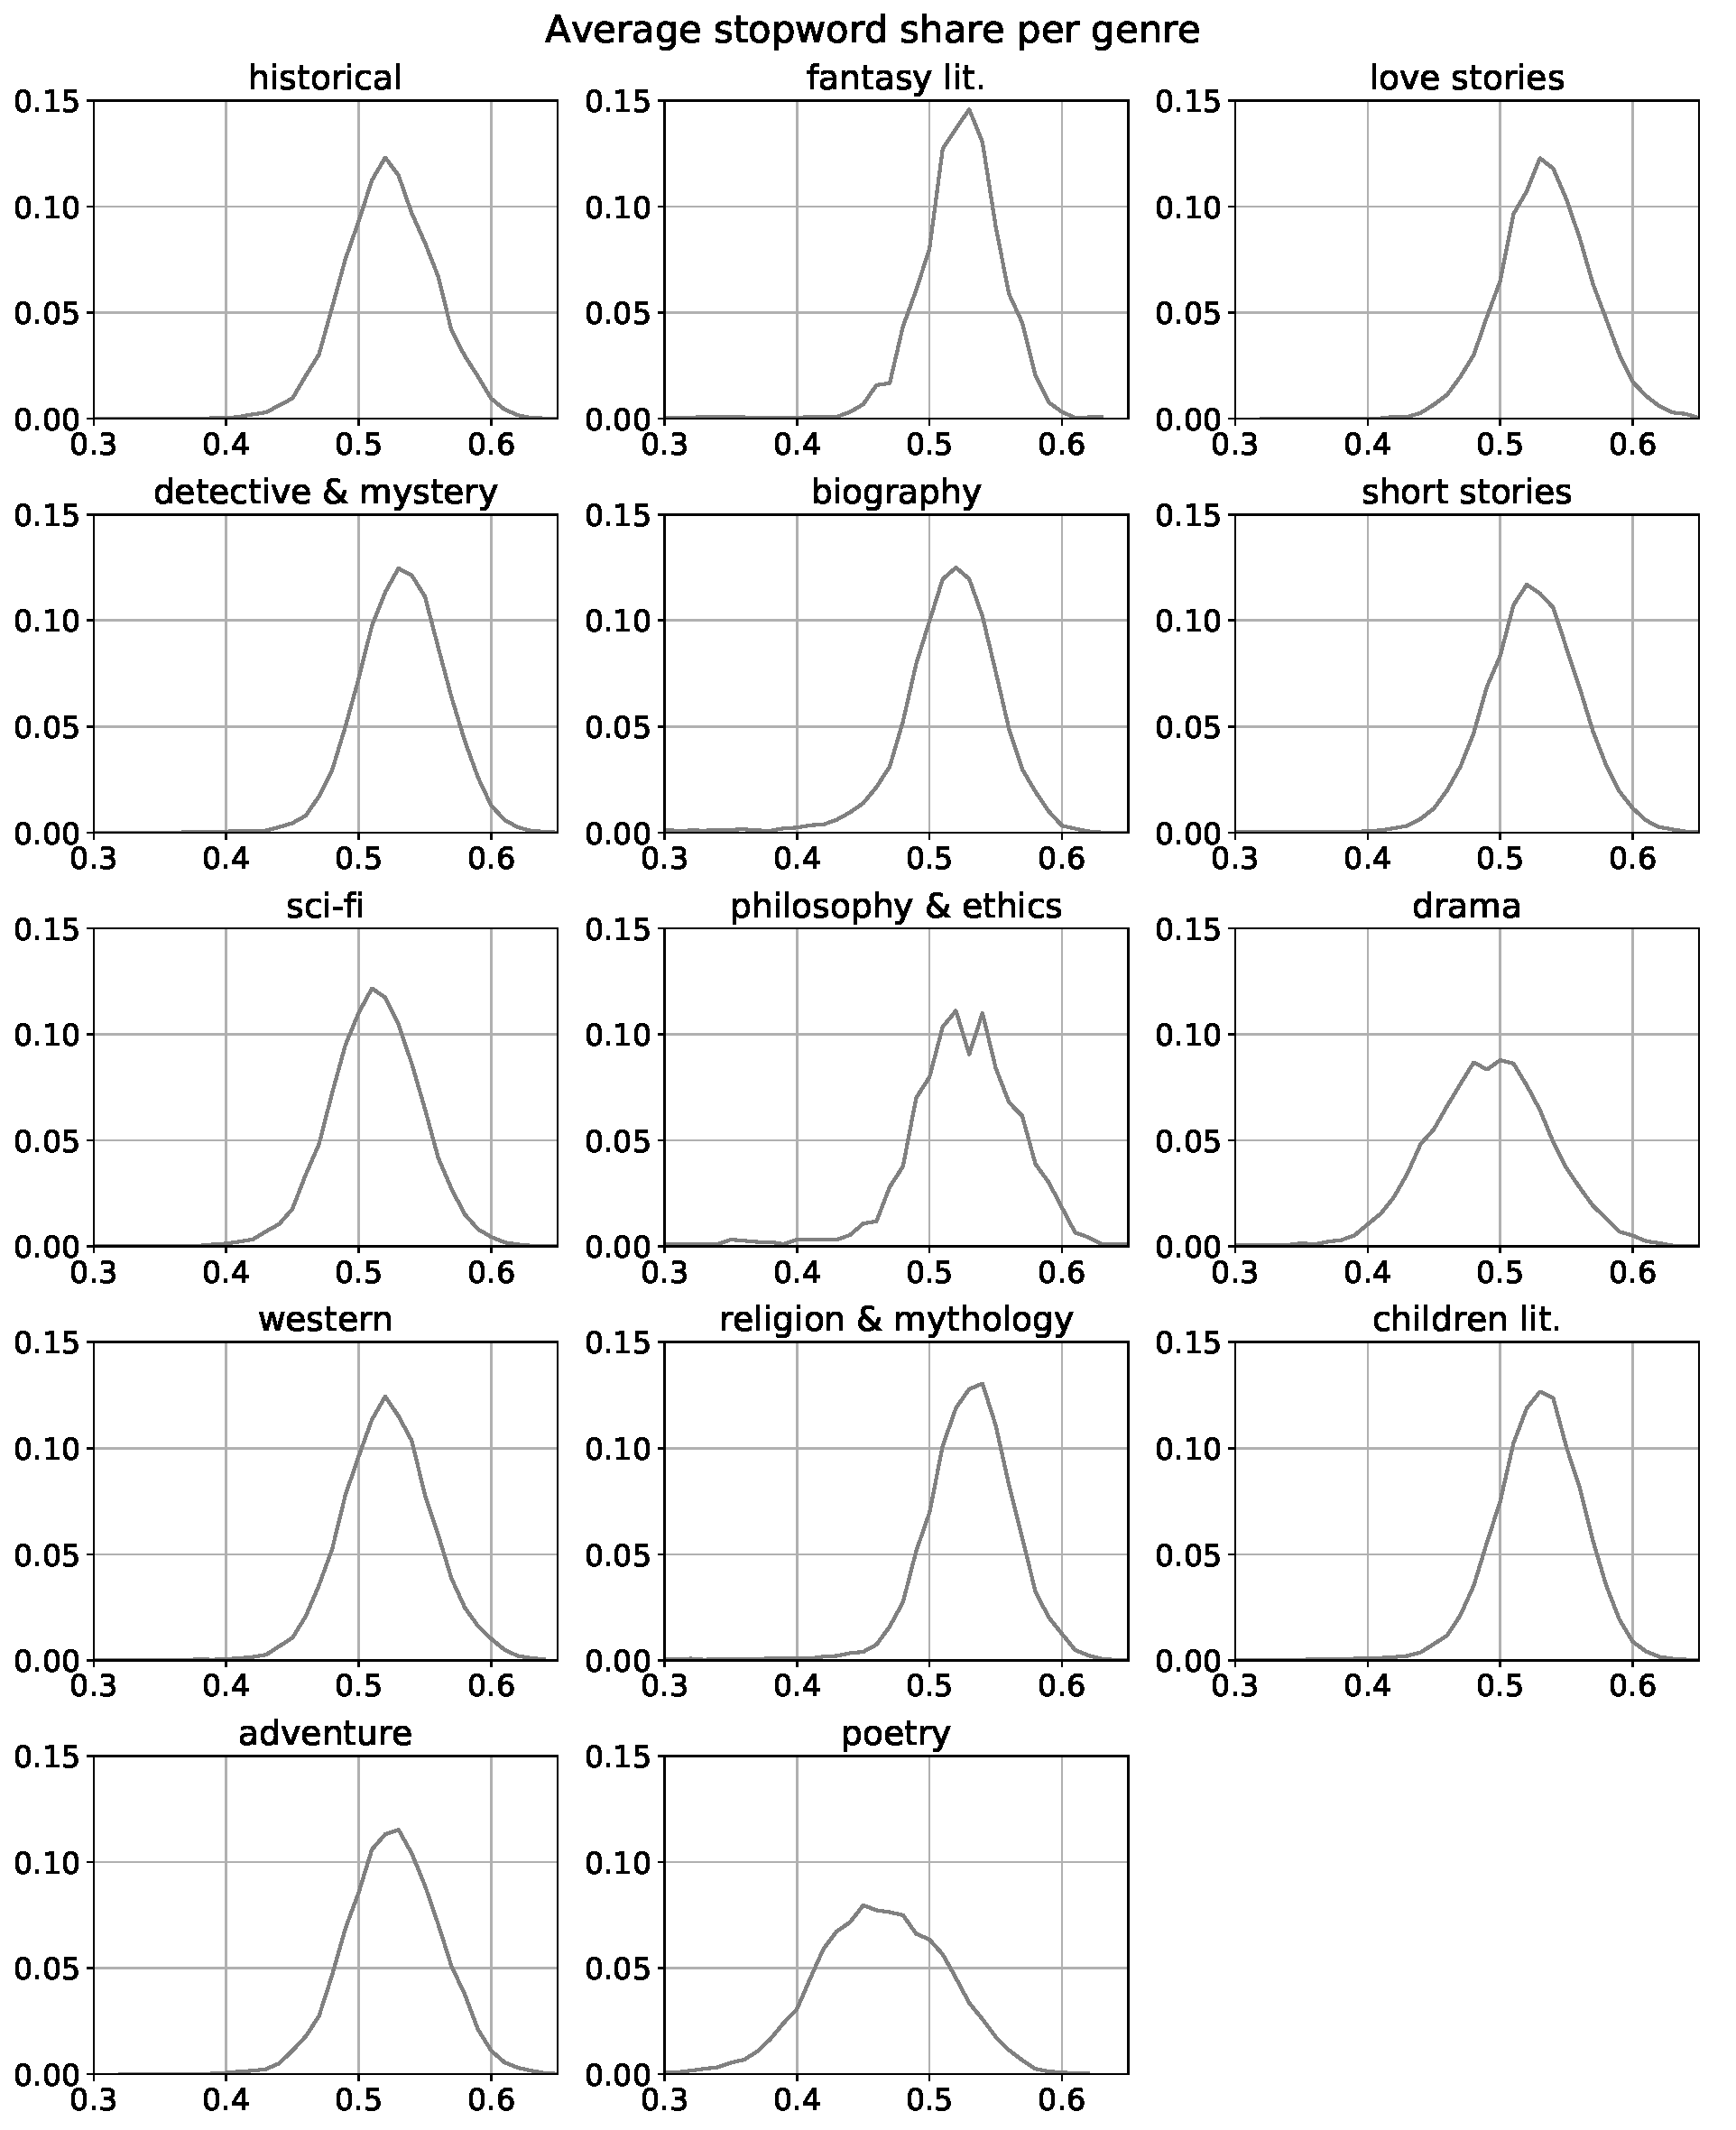
\includegraphics[height=0.4\textheight]{img/03_stopwords}
	\caption{Average stop words share per genre.}
	\label{fig:stopwords}
\end{figure}

\end{comment}



\begin{comment}
\subsubsection{Part of speech}
\end{comment}
